% Document settings
\documentclass[11pt]{article}
% % % % % % % % % % % Define Footer
\usepackage{fancyhdr}
\usepackage[margin=1in]{geometry}
\usepackage[pdftex]{graphicx}
\usepackage{multirow}
\usepackage{setspace}
\pagestyle{plain}
\usepackage[american voltages,oldvoltagedirection]{circuitikz}
%\usepackage[american]{circuitikz}
\usepackage{graphicx}
\usepackage{multirow}
\usepackage{booktabs}
\usepackage{epstopdf}
%\usepackage{MnSymbol,wasysym}
\usepackage{amsmath}
%\usepackage{mathtools}
\usepackage{amssymb}
\usepackage{lipsum}
\usepackage{siunitx}
\setlength\parindent{0pt}
\graphicspath{{images/}{drawings/}}
\usepackage{float}
% % % % % % % % % % % Header footer
% % % % % % % % % % %EDIT THIS % % % % % % % % % % % % % % % % % % % %
\pagestyle{fancy}
\fancyhf{}
\lhead{Tech Memo: Experiment 4-Operational Amplifiers}
\rhead{Andrei Tumbar}
\lfoot{EE281}
\cfoot{4/7/20}
\rfoot{Page \thepage}
% % % % % % % % % % % % % % % % % % % % % % % % % % % % % % % % % % % % %

\begin{document}
	\numberwithin{equation}{subsection}
	\numberwithin{figure}{subsection}
	\numberwithin{table}{subsection}
	\hspace{6in}
		
\includegraphics[scale=0.9,trim=0cm 0in 0in 0.0in,clip]{RIT_KGCOE1}
\newline

\Huge \textbf{EEEE 281 Experiment 4:\\ Operational Amplifiers}\\

\Large
\textbf{From:}Andrei Tumbar [Computer Engineering] \\
\textbf{To: } Section 2 TA: LJ Boone \\
\textbf{Date: } Performed: 4/7/20  Due: 4/14/20 \\
\textbf{Subject: } Lab 4-Operational Amplifiers\\
\textbf{Lab Partner(s): } N/A\\
\vspace{0.5in}
	\begin{table}[h!]
		\centering
		%\caption{Grading Table}
		%\label{Table:Grading Table 1}
		%\begin{tabular}{llllll}
		\begin{tabular}{|l||l|l|l|l|}
			\hline
			Component & Percentage of Grade   & Score \hspace{0.5in} & Comment \hspace{0.75in}  \\
			\hline
			Report Formatting & 20~\si{\percent} & & \\	 
			\hline
			\hline 
			Hand Calculation: Inverting Op-Amp & 5~\si{\percent} & & \\	 
			 \hline
		    Hand Calculation: Non-Inverting Op-Amp & 5~\si{\percent} & & \\	 
			 \hline
			PSPICE: Setup Conditions & 5~\si{\percent} & & \\	 
			 \hline
			PSPICE: Data and Figures & 10~\si{\percent} & & \\	 
			 \hline
			PSPICE: Discussion of Simulation & 15~\si{\percent} & & \\	 
			\hline
			\hline
			Hardware: Experimental Setup & 10~\si{\percent} & & \\	 
			\hline
			Hardware: Experimental Data and Tables & 10~\si{\percent} & & \\	 
			\hline
			Hardware: Discussion of Results & 20~\si{\percent} & & \\	 
			\hline
			\textbf{Total Score:}&  & & \\	 
			\hline
			\textbf{Graded By:}&  & & \\	 
			\hline
		\end{tabular}
	\end{table}
\newpage
\section*{Abstract}
%\Large \textbf{Abstract} \\
\normalsize
The abstract section should contain a summary of what was performed in the lab and should be approximately  200 words.  This should succinctly rephrase the purpose of the laboratory.  It should also refer to the data collected.  How many circuit topologies were  investigated (2 in this lab)?  What theory/data is observed for each circuit (Vin/Vout,V+/V- gain)?  Was clipping observed?  What voltage did it occur at?
\section {Introduction and Theory}
Include 1 paragraph that explains the scope of the experiment. Briefly introduce the concept of Operational Amplifiers.  What was the primary purpose of the experiment? What are the standard current and voltage made for Op-Amps?  Include a figure of the OpAmps; for simplicity you may use your PSPICE schematic with both OpAmps. 
\begin{figure}[h!]
	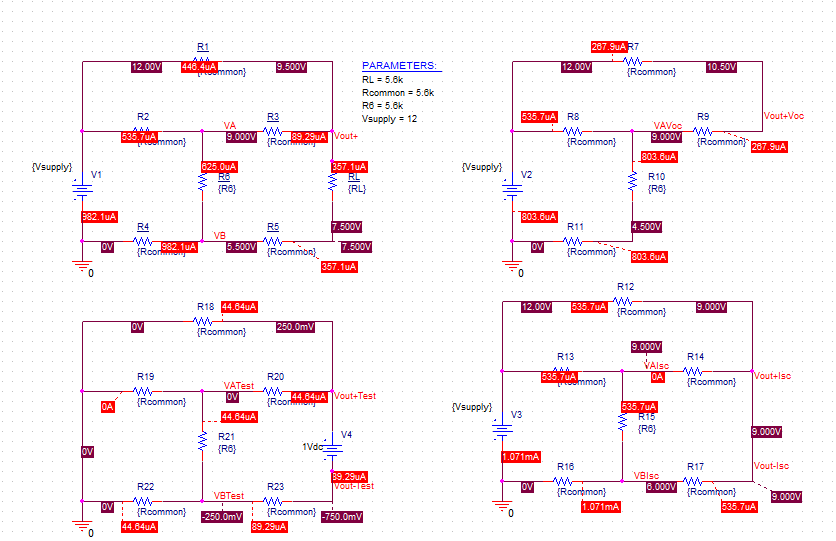
\includegraphics[width=\textwidth]{schematic_1}
	\caption{Schematic diagrams of the inverting (right) and non-inverting OpAmps used in this report. This graphic is the PSPICE schematic capture.}
	\label{Fig:PSPICEOpAmpsGraphic}
\end{figure}
\\
If the data collection has deviated in any way from the rest of your section (for example you had to come back to collect more data), explain this in a second paragraph.  In particular, be sure to note if your data was acquired from a different lab than your classmates/using different equipment. 

\subsection{Hand Calculations: Inverting Op-Amp}
\begin{itemize}
%	\item Present a figure of the inverting Op-Amp, with the value of the feedback and input resistors that you chose.   You do NOT need to include this figure a second time.
	\item Show the key steps in the derivation of the inverting Op-Amp's gain, using proper citations to the text/course notes/etc. 
	\item With a short discussion in text, justify the selection of the input resistor and feedback resistor to achieve the gain specified in the laboratory handout.  Record the values in Table \ref{Table:Lab4InvertingOpAmpSelection}
		\begin{table}[h]
			\centering
			\caption{$R_1$ and $R_f$ selection  for the Inverting Op Amp}.
			\label{Table:Lab4InvertingOpAmpSelection}
			%\begin{tabular}{llllll}
			\begin{tabular}{|c|c|c|c|}
				\hline
				$R_{in}$ (\si{\ohm})& %$I_{sc}$ (\si{\milli\ampere}) &
				$R_{f}$ (\si{\ohm}) \\
				\hline
				&   \\	 \hline 
			\end{tabular}
		\end{table}
\end{itemize}
\subsection{Hand Calculations: Non-Inverting Op-Amp}
\begin{itemize}
	%\item Present a figure of the non-inverting Op-Amp, with the value of the feedback and input resistors that you chose.   You do NOT need to include this figure a second time.
	\item Show the key steps in the derivation of the non-inverting Op-Amp's gain, using proper citations to the text/course notes/etc. 
	\item With a short discussion in text, justify the selection of the input resistor and feedback resistor to achieve the gain specified in the laboratory handout.  Record the values in Table \ref{Table:Lab4NonInvertingOpAmpSelection}.
			\begin{table}[h]
				\centering
				\caption{$R_1$ and $R_f$ selection  for the Non-Inverting Op Amp}.
				\label{Table:Lab4NonInvertingOpAmpSelection}
				%\begin{tabular}{llllll}
				\begin{tabular}{|c|c|c|c|}
					\hline
					$R_{in}$ (\si{\ohm})& %$I_{sc}$ (\si{\milli\ampere}) &
					$R_{f}$ (\si{\ohm}) \\
					\hline
					&   \\	 \hline 
				\end{tabular}
			\end{table}
\end{itemize}
\clearpage
\subsection{Theory: PSPICE Simulation Summary}
Begin by providing a 1 paragraph description of the PSPICE setup. Was a DC simulation used, transient simulation, etc.?  Which \textbf{libraries} and \textbf{PSPICE elements} were used in the simulation? You can borrow from the text of your first tech memo here.  If you do so, please be sure to cite the tech memo. Note the libraries used. You can find the information when you look at the properties of each element.  There will be a reference to a ``.olb'' file.  This is the library name. 

Include a description of the Vsin supply that was added to the circuit.  Specifically idenitify the values of the DC Offset, VAMPL, and, frequency selected.  Explain the settings used for the transient simulation.  What was the \textbf{Run to Time} value chosen to be (Note that the handout for Spring 2018 demonstrates the RunToTime parameter-how is it related to the frequency)?  Why?

\subsubsection{PSPICE Simulation: Inverting OpAmp}
\begin{itemize}
	\item Show the transient simulation for the inverting OpAmp 
	\item Make sure that the input  and output waves are clearly visible.
	\item Make the linewidth of each plot thick and clearly visible. The gain should be listed as an extracted value per the handout's tutorial.
	\item The figure caption should include: (i) the type of circuit (inverting opamp), (ii) the values of R1 and Rf, (iii) the peak to peak voltage of the output wave, and (iv) the resulting gain.  Please edit the figure caption below.
	\item \textbf{A short discussion  (3 sentences) of the figure should be included, tying it back to the hand calculations. }
\end{itemize}
\begin{figure}[h]
	\vspace{2in}
	\caption{Transient simulation of the inverting OpAmp.  The input wave had a peak-to-peak voltage of XX, the output wave had a peak-to-peak voltage of YY, and the gain was ZZ.}
\end{figure}


\subsubsection{PSPICE Simulation: Non-Inverting OpAmp}
 \begin{itemize}
 	\item Show the transient simulation for the non-inverting Op Amp 
 	\item Make sure that the input  and output waves are clearly visible.
 	\item Make the linewidth of each plot thick and clearly visible. The gain should be listed as an extracted value per the handout's tutorial.
 	\item The figure caption should include: (i) the type of circuit (non-inverting opamp), (ii) the values of R1 and Rf, (iii) the peak to peak voltage of the output wave, and (iv) the resulting gain. Please edit the figure caption below.
 	\item \textbf{A short discussion  (3 sentences) of the figure should be included, tying it back to the hand calculations. }
 \end{itemize}
\begin{figure}[h]
	\vspace{2in}
	\caption{Transient simulation of the non-inverting OpAmp.  The input wave had a peak-to-peak voltage of XX, the output wave had a peak-to-peak voltage of YY, and the gain was ZZ.}
\end{figure}


\section{Hardware Experiment: Results and Discussion}
This section of the report should present what was done in hardware.  A reader should be able to recreate an experiment from the detail present.  One section discusses the equipment used in the experiment. The remaining sections discuss the results for each circuit.
\subsection{Equipment Used in the Laboratory}
Write a short paragraph to detail the equipment used in the laboratory, and specific model numbers. Ideally, you should create a table of the equipment which should be referred to in text (See Table \ref{Table:Equipment} as an example).  The room location where the experiment was performed should be included.  Note that this should be a part of all Tech Memos, as it is an essential piece for other users to replicate your experiment.  \textbf{As you will be likely using the same equipment throughout the term, once the text/tables are established, you may reuse the information with the permission of your instructor/TA. Again, cite your first lab report as a reference.}
		
		\begin{table}[H]
			\centering
			\caption{Equipment/Software required for Lab 4.}
			\label{Table:Equipment}
			%\begin{tabular}{llllll}
			\begin{tabular}{|c||c|c|c|c|}
				\hline
				Item & Tool & Room      \\
				\hline
				Simulation & OrCAD Capture CIS & All Open EE Labs   \\	 
				\hline 
				DC Power Supply&  Agilent E3630A  & 09-3170   \\	
				\hline  
				DC Power Supply & Agilent E3631A   & 09-3200 \\ 
				\hline 
				Multimeter & Agilent E34401A   & 09-3170, 09-3200 \\ 
				\hline 
				Waveform Generator & Agilent 33120A & 09-3170, 09-3200 \\
				\hline
				Oscilloscope & Textronix TDS2012C & 09-3200  \\
				\hline
				Oscilloscope & Agilent DSO 3102A & 09-3170  \\
				\hline
			\end{tabular}
		\end{table}
\subsection{Hardware Results: Inverting Operational Amplifier}	
\begin{itemize}
	\item Include a figure showing  the Oscilloscope trace for the inverting Op Amp at the Vin and Vout. Make sure the peak to peak voltage is labeled  Make sure that the plot clearly shows the date that the picture was taken. Also, edit the caption below.
	\begin{figure}[h]
		\vspace{2in}
		\caption{Oscilloscope trace of the inverting OpAmp.  The input wave had a peak-to-peak voltage of XX, the output wave had a peak-to-peak voltage of YY, and the gain was ZZ.}
	\end{figure}
	\item Include the measurements for V+ and V- in the table. These likely were measured on the oscilloscope as the peak-to-peak voltage measurements of the noise (since they will be close to 0).  They should have been on the order of 10's of ~\si{\milli\volt}.
   \item Include measurements of the resistors used in the lab
	 \item Include the gain. 
 \item Summarize the results in Table \ref{Table:HardwareInverting}. 
 \item 	Show an oscilloscope plot that illustrates clipping in the circuit.   In the figure caption, list the value of the input voltage resulting in clipping.  Also, edit the caption below.v
 \begin{figure}[h]
 	\vspace{2in}
 	\caption{Oscilloscope trace of clipping for the inverting OpAmp.  The input wave had a peak-to-peak voltage of XX.}
 \end{figure}
 \item Include 1-2 paragraphs explaining/analyzing all of the results for this section. Perform an error analysis to PSPICE.
 \begin{table}[h!]
 	\centering
 	\caption{Table of hardware results before saturation for the inverting Op-Amp.}.
 	\label{Table:HardwareInverting}
 	%\begin{tabular}{llllll}
 	\begin{tabular}{|c||c|c|c|}
 		\hline
 		& Inverting Amplifier   \\
 		\hline
 		Non-inverting input~(\si{\volt}) &   \\	
 		(pin 3) &  \\ \hline 
 		Inverting input~(\si{\volt}) &   \\	
 		(pin 2) &  \\ \hline  
 		$R_{1}$~(\si{\ohm}) &  \\	\hline
 		$R_{f}$~(\si{\ohm}) &  \\	\hline
 		$V_{in}$ ~(\si{\volt})&   \\
 		(Waveform Generator) &  \\ \hline 
 		$V_{out}$~(\si{\volt}) &   \\
 		(pin 6) &  \\ \hline
 		$A_{d}=\frac{V_{out}}{V_{in}}$ &   \\	\hline	
 	\end{tabular}
 \end{table}
\end{itemize}

  
  \subsection{Hardware Results: Non-Inverting Operational Amplifier}
  \begin{itemize}
  	 \item	Include a figure showing  the Oscilloscope trace for the non-inverting Op Amp at the Vin and Vout. Make sure the peak to peak voltage is labeled  Make sure that the plot clearly shows the date that the picture was taken. Also, edit the caption below.
  	 	\begin{figure}[h]
  	 	\vspace{2in}
  	 	\caption{Oscilloscope trace of the non-inverting OpAmp.  The input wave had a peak-to-peak voltage of XX, the output wave had a peak-to-peak voltage of YY, and the gain was ZZ.}
  	 \end{figure}
  \item	Include the measurements for V+ and V- in the table. These likely were measured on the oscilloscope as the peak-to-peak voltage measurements of the noise (since they will be close to 1).  
  \item	Include measurements of the resistors used in the lab
  \item	Include the gain. 
  \item	Summarize the results for  in Table \ref{Table:HardwareNonInverting}.
  \item	Show an oscilloscope plot that illustrates clipping in the circuit.   In the figure caption, list the value of the input voltage resulting in clipping.  Also, edit the caption below.
   \begin{figure}[h]
  	\vspace{2in}
  	\caption{Oscilloscope trace of clipping for the non-inverting OpAmp.  The input wave had a peak-to-peak voltage of XX.}
  \end{figure}
   \item Include 1-2 paragraphs explaining/analyzing all of the results for this section. Perform an error analysis.
  \end{itemize}
\begin{table}[h!]
	\centering
	\caption{Table of hardware results before saturation for the non-inverting Op-Amp.}.
	\label{Table:HardwareNonInverting}
	%\begin{tabular}{llllll}
	\begin{tabular}{|c||c|c|c|}
		\hline
		& Non-Inverting Amplifier   \\
		\hline
		Non-inverting input~(\si{\volt}) &   \\	
		(pin 3) &  \\ \hline 
		Inverting input~(\si{\volt}) &   \\	
		(pin 2) &  \\ \hline  
		$R_{1}$~(\si{\ohm}) &  \\	\hline
		$R_{f}$~(\si{\ohm}) &  \\	\hline
		$V_{in}$ ~(\si{\volt})&   \\	
		(Waveform Generator) &  \\ \hline 
		$V_{out}$~(\si{\volt}) &   \\	
		(pin 6) &  \\ \hline
		$A_{d}=\frac{V_{out}}{V_{in}}$ &   \\	\hline		
	\end{tabular}
\end{table}
	\section{Conclusion}
	Provide a 1 paragraph summary of the laboratory experiment.  What were the major conclusions for each part of the experiment?  Also did the theory agree with the experiment?  The conclusion is a revised version of the abstract. Some specific verbiage from the lab documentation lists the following points:
\begin{itemize}
		\item Include a concise statement of conclusions commenting on differences, if any, between the ideal and simulated performance of the circuit and theory. 
		\item  Does the data agree with the hand calculations and PSPICE simulations? Why does clipping occur (discuss)? How would the voltage resulting in onset of clipping change if the power supply was adjusted to +/- 15 volts for both configurations.
\end{itemize}	
	\section{Acknowledgments}
	Acknowledge \textbf{any} source of help received in the experiment/writing the report.  This should certainly include your lab partner/teaching assistant/instructor.  It may also include other classmates/study partners. State briefly what the nature of the help was.
	
	\textbf{Your report should include references to appropriate pages in the text, as well as any other sources, websites/etc. consulted in the preparation of the report.}
\begin{thebibliography}{9}
	\bibitem{AlexanderSadiku}
	C.K. Alexander, and M.K.O. Sadiku,
	\emph{Fundamentals of Electric Circuits, 4th Edition},
	McGraw Hill, pp. xx-yy(EDIT), 2009.
	\bibitem{OldLab}
A. Student,
	\emph{EEEE 281 Lab 1 Tech Memo},
	page xx-yy, submitted Month, Day, 2015.
	\bibitem{RommelLab}
	S. Rommel,
	\emph{EEEE 281 Lab 1 Lecture notes},
	slides xx-yy, Spring 2015.
\end{thebibliography}

\end{document}



